%!TEX root = /Users/stevenmartell/Documents/CONSULTING/HumpbackChub/HBC_2011_Assessment/WRITEUP/HBCmain.tex


\subsection{Annual growth rates from capture-recapture information} % (fold)
\label{sub:annual_growth_rates_from_capture_recapture_information}

Parameters for the von Bertalanffy growth model were estimated from the annual growth increment data, where the data were restricted to measured individuals recaptured in the subsequent year (Figure \ref{fig:FIGS_LSMR_fig:AnnualGrowthIncrements}).  The fitted growth model assumed a measurement error with a standard deviation equal to 9.14 mm.  This measurement error was based on the standard deviation in total length of individuals captured multiple times within a 20-day period (roughly the duration of a sampling trip).  Quantile regressions on the raw annual growth increment data (Figure \ref{fig:FIGS_LSMR_fig:AnnualGrowthIncrements}) indicate a steeper, more negative, slope in recent years.  Or in other words, annual growth rates have been increasing in recent years.



\begin{figure}[htbp]
	\centering
		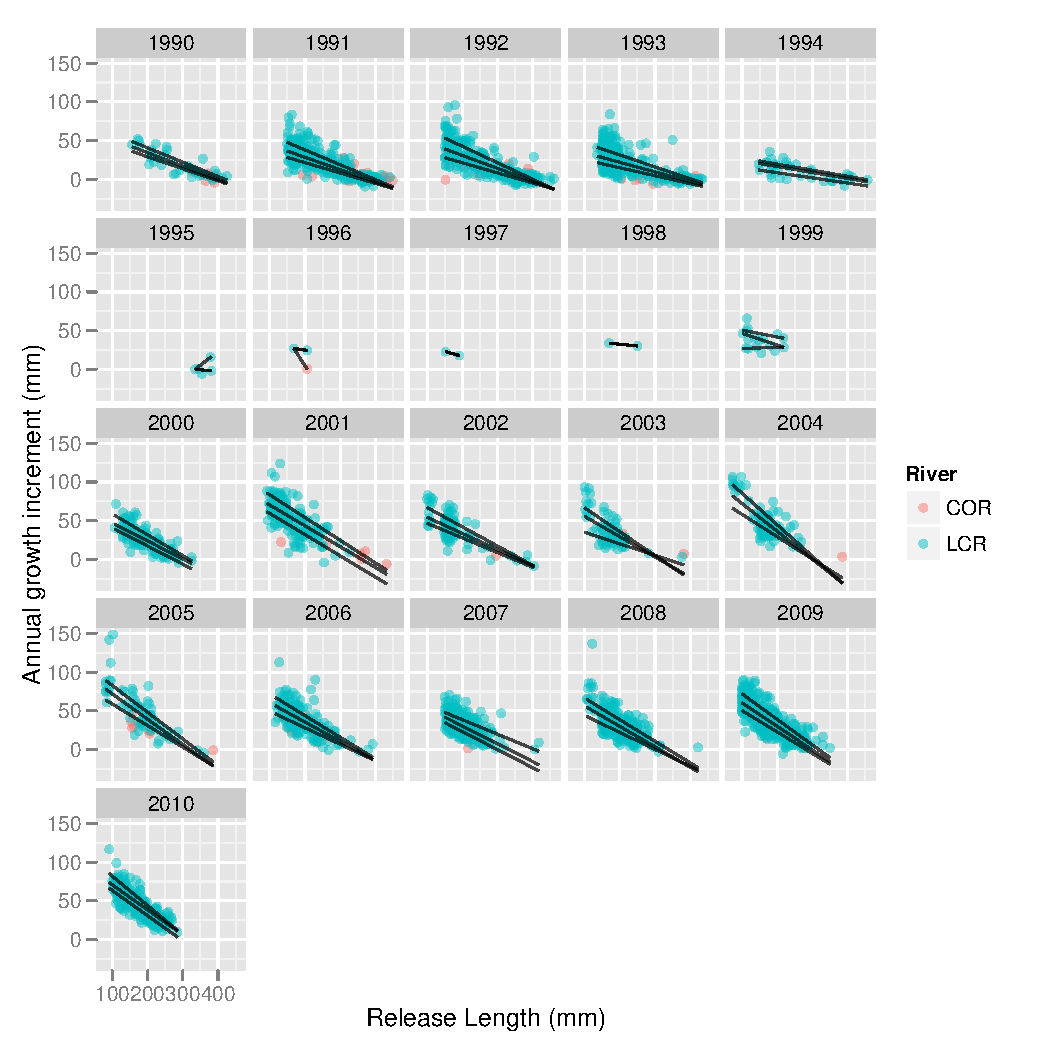
\includegraphics[width=6.5in]{../FIGS/LSMR/fig:GrowthIncrements.pdf}
	\caption{Growth increments by tag year for individually tagged humpback chub that have been at large for at least 1 year.   Recapture events could have occurred in either river. Fitted lines correspond to the 5, 50 and 95 percentiles of the data.}
	\label{fig:FIGS_LSMR_fig:GrowthIncrements}
\end{figure}

\begin{figure}[htbp]
	\centering
		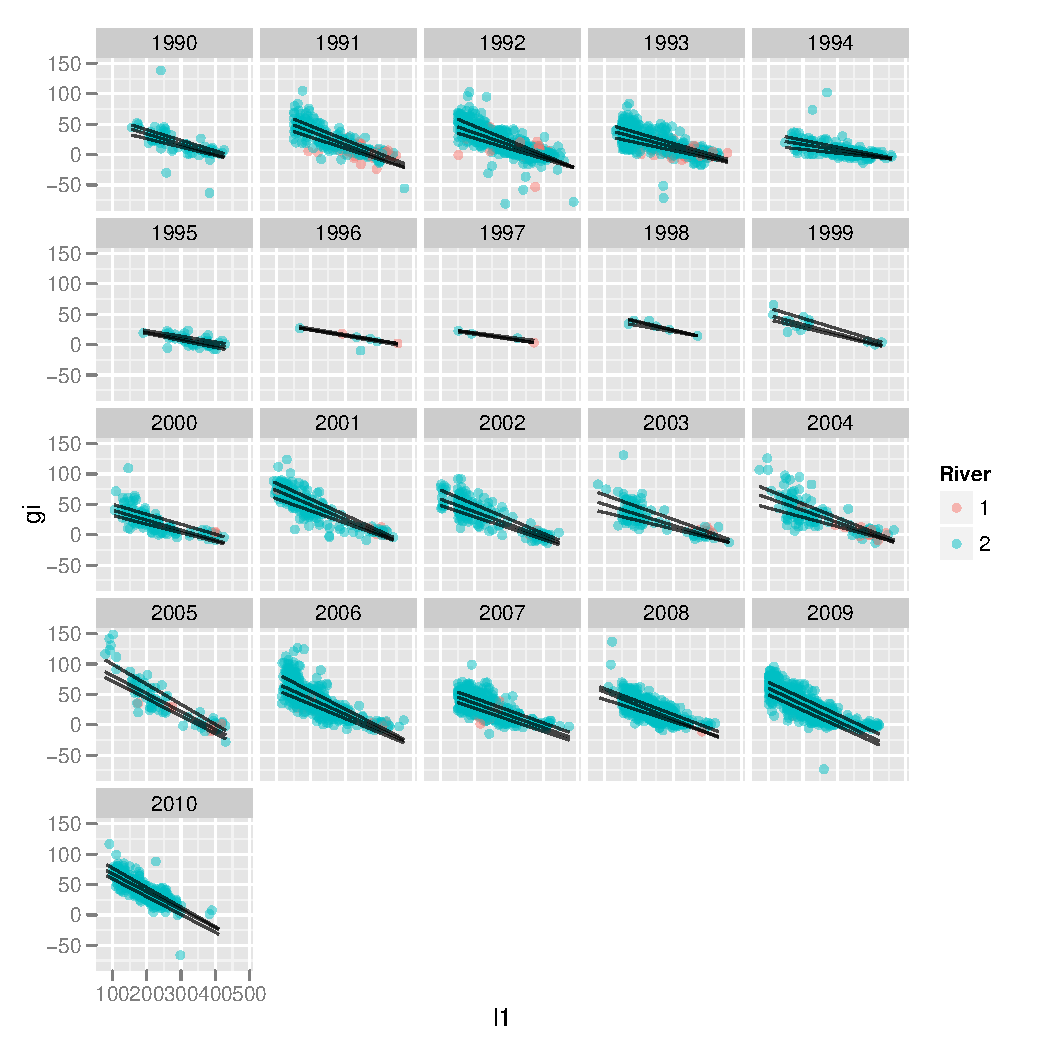
\includegraphics[width=6.5in]{../FIGS/LSMR/fig:AnnualGrowthIncrements.pdf}
	\caption{Annual growth increments of humpback chub of all fish captured and recaptured in the following year. River 2 corresponds to fish tagged in the Little Colorado River, River 1 the Colorado River. Fitted lines correspond to the 5, 50 and 95 percentiles of the data.}
	\label{fig:FIGS_LSMR_fig:AnnualGrowthIncrements}
\end{figure}

Estimated growth parameters based on the annual growth increment data are shown in Figure \ref{fig:FIGS_LSMR_fig:LinfPosteriors}.  Sample sizes between 1995 and 1999 were extremely small and are reflected in the uncertainty in estimates of asymptotic length and $k$.  The median estimate of $l_\infty$ over the entire time series is 373.4 mm with a standard deviation of 28.88 mm.  The overall median estimate of $k$ is 0.246 with a standard deviation of 0.106.  In 2005, the median estimate of $k$ (0.536) was more than twice as large as the overall median estimate owing to the a number of individual fish that were less than 100 mm in 2004 having a growth increment of more than 100 mm in a single year (Figure \ref{fig:FIGS_LSMR_fig:AnnualGrowthIncrements}, year 2005 panel).

\begin{figure}[htbp]
	\centering
		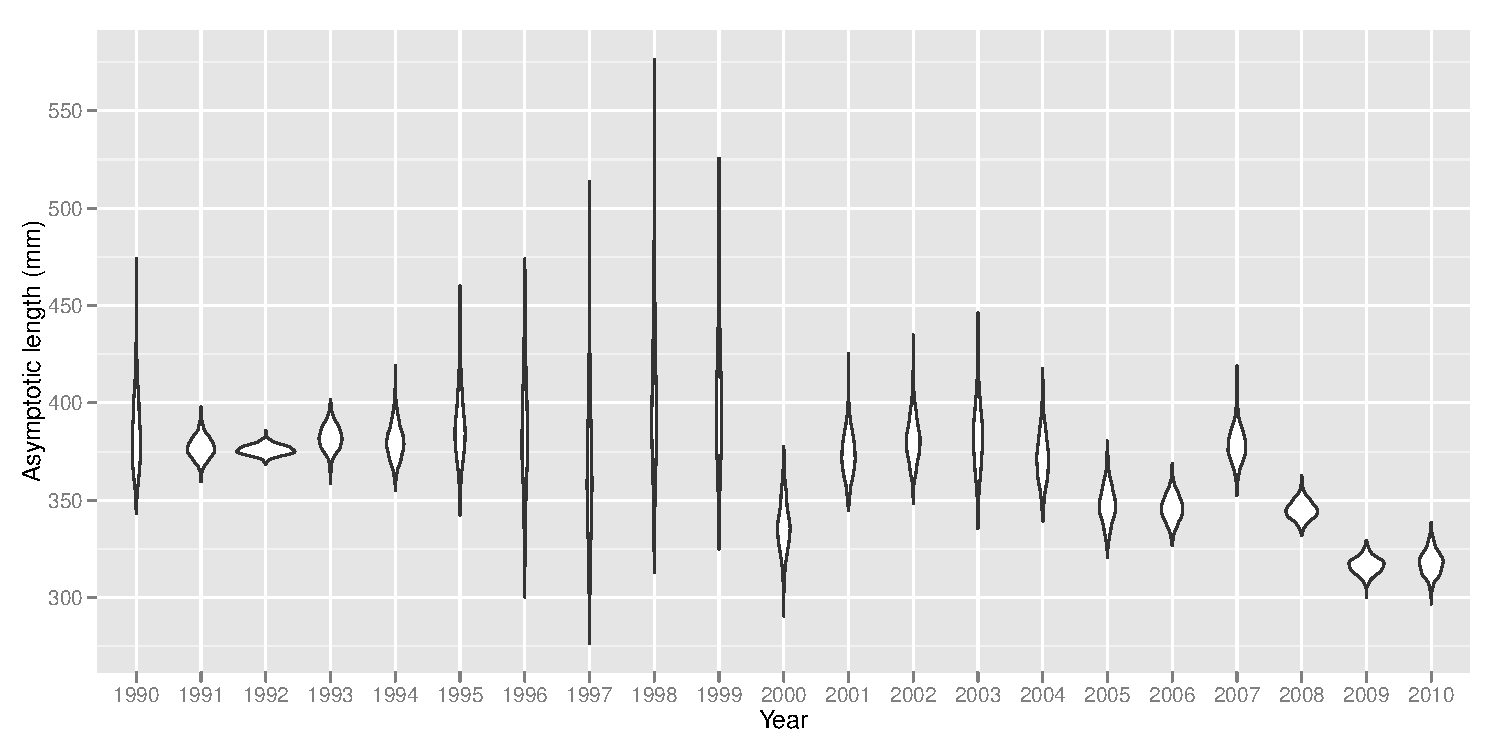
\includegraphics[width=6.5in]{../FIGS/LSMR/fig:LinfPosteriors.pdf}
		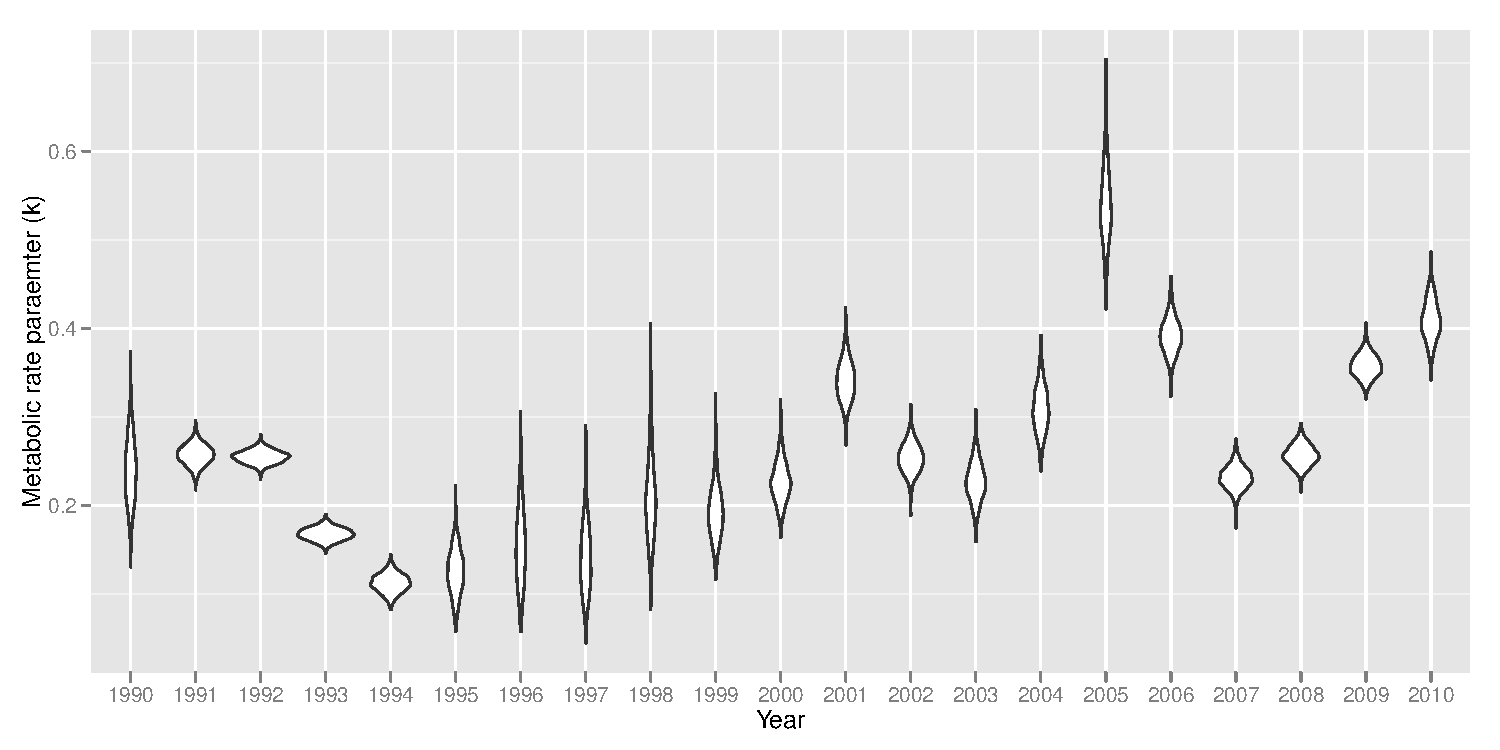
\includegraphics[width=6.5in]{../FIGS/LSMR/fig:kPosteriors.pdf}
	\caption{Violin plots of the marginal posterior distributions for annual estimates of asymptotic length ($l_\infty$, top panel) and the von Bertalanffy metabolic rate parameter ($k$).}
	\label{fig:FIGS_LSMR_fig:LinfPosteriors}
\end{figure}

Estimated growth transition matrices based on the estimated growth parameters from the annual growth increment data are shown in Figure \ref{fig:FIGS_LSMR_fig:TransitionMatrix}. In addition to the transition matrix based, this Figure also has a 1:1 reference line and the corresponding maximum likelihood estimate of $l_\infty$ as a reference to judge differences in the annual length transition matrices.  Starting 2001, growth rates of fish less than 150 mm increased markedly relative to the growth increments observed in the 1990s.  The implications of this increased growth rate in a length-based model would have significant impacts on annual recruitment estimates if growth was assumed to be constant.  The length transition matrices shown in Figure \ref{fig:FIGS_LSMR_fig:TransitionMatrix} provide an alternative input into the length structured mark recapture model (LSMR), where length-transition matrices are estimated externally.


\begin{figure}[htbp]
	\centering
		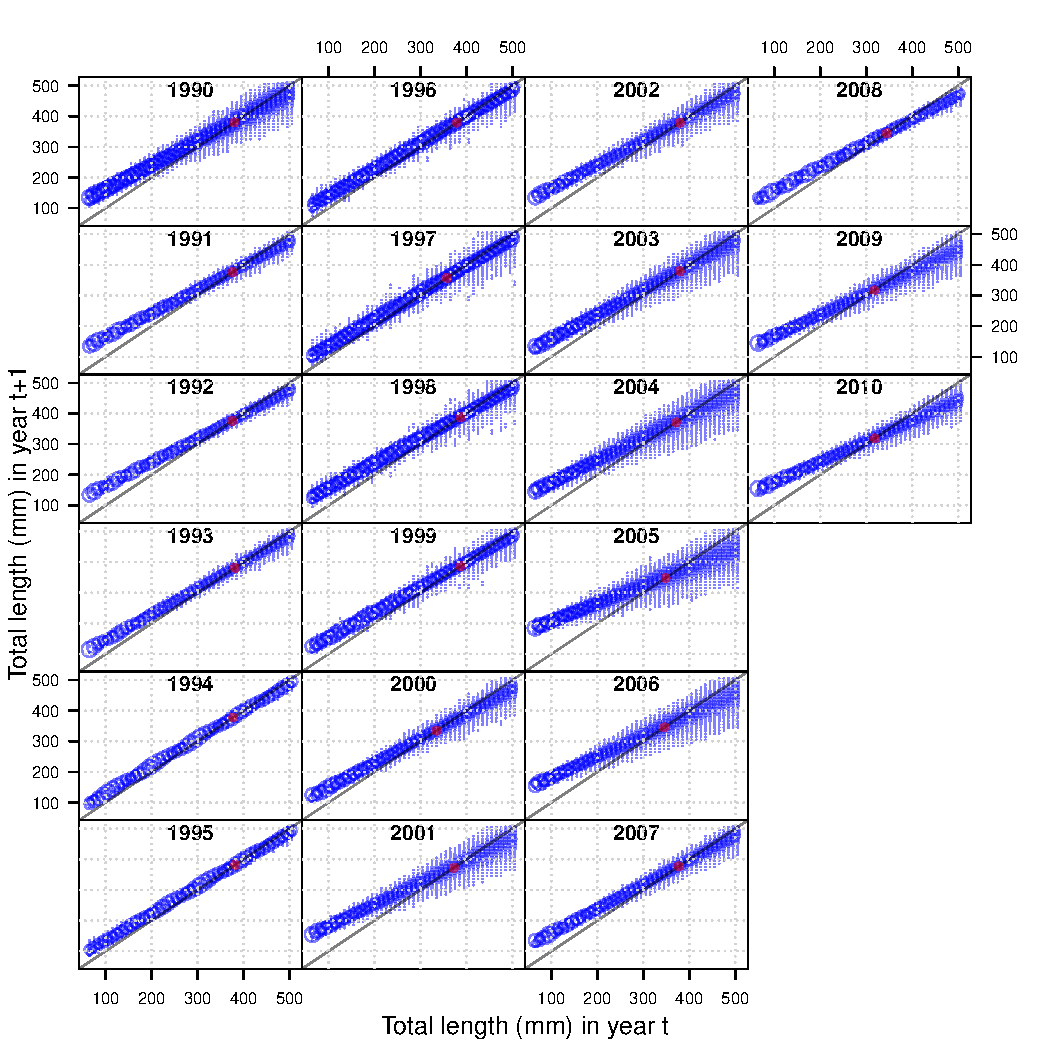
\includegraphics[width=6.5in]{../FIGS/LSMR/fig:TransitionMatrix.pdf}
	\caption{Annual length transition matrixes based on the annual growth increment data.  The area of each bubble is proportional to the transition probability from year $t$ to year $t+1$, the diagonal black line is the 1:1 slope, and the red circle corresponds to the maximum likelihood estimate of $l_\infty$.  Each matrix is based on parametric uncertainty in the estimated von Bertalanffy growth parameters as well as measurement errors. }
	\label{fig:FIGS_LSMR_fig:TransitionMatrix}
\end{figure}


% subsection annual_growth_rates_from_capture_recapture_information (end)
